\panel{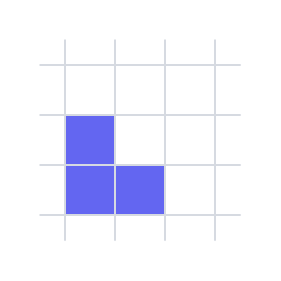
\begin{tikzpicture}[x=1bp, y=1bp]\path[use as bounding box] (0,0) rectangle (81.00,81.00);\clip (0,0) rectangle (81.00,81.00);
\path[fill={rgb,255:red,99;green,102;blue,241}] (31.50,13.50) rectangle (49.50,31.50);
\path[fill={rgb,255:red,99;green,102;blue,241}] (13.50,31.50) rectangle (31.50,49.50);
\path[fill={rgb,255:red,99;green,102;blue,241}] (13.50,13.50) rectangle (31.50,31.50);
\path[draw={rgb,255:red,214;green,218;blue,225}, line width=0.68bp, line cap=round, line join=round] (13.50,4.50) -- (13.50,76.50);
\path[draw={rgb,255:red,214;green,218;blue,225}, line width=0.68bp, line cap=round, line join=round] (31.50,4.50) -- (31.50,76.50);
\path[draw={rgb,255:red,214;green,218;blue,225}, line width=0.68bp, line cap=round, line join=round] (49.50,4.50) -- (49.50,76.50);
\path[draw={rgb,255:red,214;green,218;blue,225}, line width=0.68bp, line cap=round, line join=round] (67.50,4.50) -- (67.50,76.50);
\path[draw={rgb,255:red,214;green,218;blue,225}, line width=0.68bp, line cap=round, line join=round] (4.50,13.50) -- (76.50,13.50);
\path[draw={rgb,255:red,214;green,218;blue,225}, line width=0.68bp, line cap=round, line join=round] (4.50,31.50) -- (76.50,31.50);
\path[draw={rgb,255:red,214;green,218;blue,225}, line width=0.68bp, line cap=round, line join=round] (4.50,49.50) -- (76.50,49.50);
\path[draw={rgb,255:red,214;green,218;blue,225}, line width=0.68bp, line cap=round, line join=round] (4.50,67.50) -- (76.50,67.50);
\end{tikzpicture}}{(a) $S$: $m = 3$, $r = 2$, $c = 2$}\hspace{16.5bp}\panel{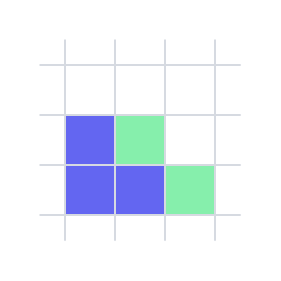
\begin{tikzpicture}[x=1bp, y=1bp]\path[use as bounding box] (0,0) rectangle (81.00,81.00);\clip (0,0) rectangle (81.00,81.00);
\path[fill={rgb,255:red,99;green,102;blue,241}] (31.50,13.50) rectangle (49.50,31.50);
\path[fill={rgb,255:red,99;green,102;blue,241}] (13.50,31.50) rectangle (31.50,49.50);
\path[fill={rgb,255:red,99;green,102;blue,241}] (13.50,13.50) rectangle (31.50,31.50);
\path[fill={rgb,255:red,134;green,239;blue,172}] (31.50,31.50) rectangle (49.50,49.50);
\path[fill={rgb,255:red,134;green,239;blue,172}] (49.50,13.50) rectangle (67.50,31.50);
\path[draw={rgb,255:red,214;green,218;blue,225}, line width=0.68bp, line cap=round, line join=round] (13.50,4.50) -- (13.50,76.50);
\path[draw={rgb,255:red,214;green,218;blue,225}, line width=0.68bp, line cap=round, line join=round] (31.50,4.50) -- (31.50,76.50);
\path[draw={rgb,255:red,214;green,218;blue,225}, line width=0.68bp, line cap=round, line join=round] (49.50,4.50) -- (49.50,76.50);
\path[draw={rgb,255:red,214;green,218;blue,225}, line width=0.68bp, line cap=round, line join=round] (67.50,4.50) -- (67.50,76.50);
\path[draw={rgb,255:red,214;green,218;blue,225}, line width=0.68bp, line cap=round, line join=round] (4.50,13.50) -- (76.50,13.50);
\path[draw={rgb,255:red,214;green,218;blue,225}, line width=0.68bp, line cap=round, line join=round] (4.50,31.50) -- (76.50,31.50);
\path[draw={rgb,255:red,214;green,218;blue,225}, line width=0.68bp, line cap=round, line join=round] (4.50,49.50) -- (76.50,49.50);
\path[draw={rgb,255:red,214;green,218;blue,225}, line width=0.68bp, line cap=round, line join=round] (4.50,67.50) -- (76.50,67.50);
\end{tikzpicture}}{add the right shift: 2 new}\hspace{16.5bp}\panel{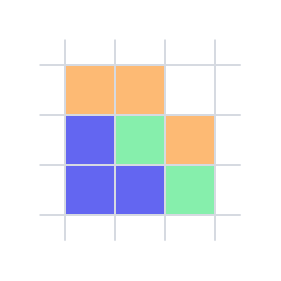
\begin{tikzpicture}[x=1bp, y=1bp]\path[use as bounding box] (0,0) rectangle (81.00,81.00);\clip (0,0) rectangle (81.00,81.00);
\path[fill={rgb,255:red,99;green,102;blue,241}] (31.50,13.50) rectangle (49.50,31.50);
\path[fill={rgb,255:red,99;green,102;blue,241}] (13.50,31.50) rectangle (31.50,49.50);
\path[fill={rgb,255:red,99;green,102;blue,241}] (13.50,13.50) rectangle (31.50,31.50);
\path[fill={rgb,255:red,134;green,239;blue,172}] (31.50,31.50) rectangle (49.50,49.50);
\path[fill={rgb,255:red,134;green,239;blue,172}] (49.50,13.50) rectangle (67.50,31.50);
\path[fill={rgb,255:red,253;green,186;blue,116}] (13.50,49.50) rectangle (31.50,67.50);
\path[fill={rgb,255:red,253;green,186;blue,116}] (31.50,49.50) rectangle (49.50,67.50);
\path[fill={rgb,255:red,253;green,186;blue,116}] (49.50,31.50) rectangle (67.50,49.50);
\path[draw={rgb,255:red,214;green,218;blue,225}, line width=0.68bp, line cap=round, line join=round] (13.50,4.50) -- (13.50,76.50);
\path[draw={rgb,255:red,214;green,218;blue,225}, line width=0.68bp, line cap=round, line join=round] (31.50,4.50) -- (31.50,76.50);
\path[draw={rgb,255:red,214;green,218;blue,225}, line width=0.68bp, line cap=round, line join=round] (49.50,4.50) -- (49.50,76.50);
\path[draw={rgb,255:red,214;green,218;blue,225}, line width=0.68bp, line cap=round, line join=round] (67.50,4.50) -- (67.50,76.50);
\path[draw={rgb,255:red,214;green,218;blue,225}, line width=0.68bp, line cap=round, line join=round] (4.50,13.50) -- (76.50,13.50);
\path[draw={rgb,255:red,214;green,218;blue,225}, line width=0.68bp, line cap=round, line join=round] (4.50,31.50) -- (76.50,31.50);
\path[draw={rgb,255:red,214;green,218;blue,225}, line width=0.68bp, line cap=round, line join=round] (4.50,49.50) -- (76.50,49.50);
\path[draw={rgb,255:red,214;green,218;blue,225}, line width=0.68bp, line cap=round, line join=round] (4.50,67.50) -- (76.50,67.50);
\end{tikzpicture}}{add the up shift: 3 new}\hspace{16.5bp}\panel{\begin{tikzpicture}[x=1bp, y=1bp]\path[use as bounding box] (0,0) rectangle (114.30,114.30);\clip (0,0) rectangle (114.30,114.30);
\path[fill={rgb,255:red,203;green,213;blue,225}] (8.40,8.40) rectangle (27.90,27.90);
\path[fill={rgb,255:red,203;green,213;blue,225}] (8.40,47.40) rectangle (27.90,66.90);
\path[fill={rgb,255:red,203;green,213;blue,225}] (8.40,86.40) rectangle (27.90,105.90);
\path[fill={rgb,255:red,203;green,213;blue,225}] (27.90,27.90) rectangle (47.40,47.40);
\path[fill={rgb,255:red,203;green,213;blue,225}] (27.90,66.90) rectangle (47.40,86.40);
\path[fill={rgb,255:red,203;green,213;blue,225}] (47.40,8.40) rectangle (66.90,27.90);
\path[fill={rgb,255:red,203;green,213;blue,225}] (47.40,47.40) rectangle (66.90,66.90);
\path[fill={rgb,255:red,203;green,213;blue,225}] (47.40,86.40) rectangle (66.90,105.90);
\path[fill={rgb,255:red,203;green,213;blue,225}] (66.90,27.90) rectangle (86.40,47.40);
\path[fill={rgb,255:red,203;green,213;blue,225}] (66.90,66.90) rectangle (86.40,86.40);
\path[fill={rgb,255:red,203;green,213;blue,225}] (86.40,8.40) rectangle (105.90,27.90);
\path[fill={rgb,255:red,203;green,213;blue,225}] (86.40,47.40) rectangle (105.90,66.90);
\path[fill={rgb,255:red,203;green,213;blue,225}] (86.40,86.40) rectangle (105.90,105.90);
\path[draw={rgb,255:red,148;green,163;blue,184}, line width=0.68bp, line cap=round, line join=round] (8.40,4.50) -- (8.40,109.80);
\path[draw={rgb,255:red,148;green,163;blue,184}, line width=0.68bp, line cap=round, line join=round] (27.90,4.50) -- (27.90,109.80);
\path[draw={rgb,255:red,148;green,163;blue,184}, line width=0.68bp, line cap=round, line join=round] (47.40,4.50) -- (47.40,109.80);
\path[draw={rgb,255:red,148;green,163;blue,184}, line width=0.68bp, line cap=round, line join=round] (66.90,4.50) -- (66.90,109.80);
\path[draw={rgb,255:red,148;green,163;blue,184}, line width=0.68bp, line cap=round, line join=round] (86.40,4.50) -- (86.40,109.80);
\path[draw={rgb,255:red,148;green,163;blue,184}, line width=0.68bp, line cap=round, line join=round] (105.90,4.50) -- (105.90,109.80);
\path[draw={rgb,255:red,148;green,163;blue,184}, line width=0.68bp, line cap=round, line join=round] (4.50,8.40) -- (109.80,8.40);
\path[draw={rgb,255:red,148;green,163;blue,184}, line width=0.68bp, line cap=round, line join=round] (4.50,27.90) -- (109.80,27.90);
\path[draw={rgb,255:red,148;green,163;blue,184}, line width=0.68bp, line cap=round, line join=round] (4.50,47.40) -- (109.80,47.40);
\path[draw={rgb,255:red,148;green,163;blue,184}, line width=0.68bp, line cap=round, line join=round] (4.50,66.90) -- (109.80,66.90);
\path[draw={rgb,255:red,148;green,163;blue,184}, line width=0.68bp, line cap=round, line join=round] (4.50,86.40) -- (109.80,86.40);
\path[draw={rgb,255:red,148;green,163;blue,184}, line width=0.68bp, line cap=round, line join=round] (4.50,105.90) -- (109.80,105.90);
\path[fill={rgb,255:red,99;green,102;blue,241}] (47.40,47.40) rectangle (66.90,66.90);
\path[fill={rgb,255:red,245;green,158;blue,11}] (37.65,57.15) circle[radius=3.75bp];
\path[fill={rgb,255:red,245;green,158;blue,11}] (76.65,57.15) circle[radius=3.75bp];
\path[fill={rgb,255:red,245;green,158;blue,11}] (57.15,37.65) circle[radius=3.75bp];
\path[fill={rgb,255:red,245;green,158;blue,11}] (57.15,76.65) circle[radius=3.75bp];
\path[draw={rgb,255:red,180;green,83;blue,9}, line width=1.20bp, dash pattern=on 3.00bp off 2.25bp, line join=round] (37.65,57.15) -- (57.15,76.65) -- (76.65,57.15) -- (57.15,37.65) -- cycle;
\path[draw={rgb,255:red,31;green,41;blue,55}, line width=1.20bp, -{Triangle[length=6.7bp, width=6.7bp]}, line cap=round, line join=round] (18.15,18.15) -- (37.65,37.65);
\node[anchor=base west, text={rgb,255:red,31;green,41;blue,55}, font=\fontsize{9.8}{11.7}\selectfont\sffamily\bfseries\itshape, fill=white, fill opacity=0.85, text opacity=1, inner sep=1pt] at (40.65,28.65) {u};
\path[draw={rgb,255:red,31;green,41;blue,55}, line width=1.20bp, -{Triangle[length=6.7bp, width=6.7bp]}, line cap=round, line join=round] (18.15,96.15) -- (37.65,76.65);
\node[anchor=base west, text={rgb,255:red,31;green,41;blue,55}, font=\fontsize{9.8}{11.7}\selectfont\sffamily\bfseries\itshape, fill=white, fill opacity=0.85, text opacity=1, inner sep=1pt] at (40.65,79.65) {v};
\end{tikzpicture}}{(b) a dark cell's 4 neighbors}
